\documentclass[twoside]{book}

% Packages required by doxygen
\usepackage{fixltx2e}
\usepackage{calc}
\usepackage{doxygen}
\usepackage[export]{adjustbox} % also loads graphicx
\usepackage{graphicx}
\usepackage[utf8]{inputenc}
\usepackage{makeidx}
\usepackage{multicol}
\usepackage{multirow}
\PassOptionsToPackage{warn}{textcomp}
\usepackage{textcomp}
\usepackage[nointegrals]{wasysym}
\usepackage[table]{xcolor}

% Font selection
\usepackage[T1]{fontenc}
\usepackage[scaled=.90]{helvet}
\usepackage{courier}
\usepackage{amssymb}
\usepackage{sectsty}
\renewcommand{\familydefault}{\sfdefault}
\allsectionsfont{%
  \fontseries{bc}\selectfont%
  \color{darkgray}%
}
\renewcommand{\DoxyLabelFont}{%
  \fontseries{bc}\selectfont%
  \color{darkgray}%
}
\newcommand{\+}{\discretionary{\mbox{\scriptsize$\hookleftarrow$}}{}{}}

% Page & text layout
\usepackage{geometry}
\geometry{%
  a4paper,%
  top=2.5cm,%
  bottom=2.5cm,%
  left=2.5cm,%
  right=2.5cm%
}
\tolerance=750
\hfuzz=15pt
\hbadness=750
\setlength{\emergencystretch}{15pt}
\setlength{\parindent}{0cm}
\setlength{\parskip}{3ex plus 2ex minus 2ex}
\makeatletter
\renewcommand{\paragraph}{%
  \@startsection{paragraph}{4}{0ex}{-1.0ex}{1.0ex}{%
    \normalfont\normalsize\bfseries\SS@parafont%
  }%
}
\renewcommand{\subparagraph}{%
  \@startsection{subparagraph}{5}{0ex}{-1.0ex}{1.0ex}{%
    \normalfont\normalsize\bfseries\SS@subparafont%
  }%
}
\makeatother

% Headers & footers
\usepackage{fancyhdr}
\pagestyle{fancyplain}
\fancyhead[LE]{\fancyplain{}{\bfseries\thepage}}
\fancyhead[CE]{\fancyplain{}{}}
\fancyhead[RE]{\fancyplain{}{\bfseries\leftmark}}
\fancyhead[LO]{\fancyplain{}{\bfseries\rightmark}}
\fancyhead[CO]{\fancyplain{}{}}
\fancyhead[RO]{\fancyplain{}{\bfseries\thepage}}
\fancyfoot[LE]{\fancyplain{}{}}
\fancyfoot[CE]{\fancyplain{}{}}
\fancyfoot[RE]{\fancyplain{}{\bfseries\scriptsize Generated by Doxygen }}
\fancyfoot[LO]{\fancyplain{}{\bfseries\scriptsize Generated by Doxygen }}
\fancyfoot[CO]{\fancyplain{}{}}
\fancyfoot[RO]{\fancyplain{}{}}
\renewcommand{\footrulewidth}{0.4pt}
\renewcommand{\chaptermark}[1]{%
  \markboth{#1}{}%
}
\renewcommand{\sectionmark}[1]{%
  \markright{\thesection\ #1}%
}

% Indices & bibliography
\usepackage{natbib}
\usepackage[titles]{tocloft}
\setcounter{tocdepth}{3}
\setcounter{secnumdepth}{5}
\makeindex

% Hyperlinks (required, but should be loaded last)
\usepackage{ifpdf}
\ifpdf
  \usepackage[pdftex,pagebackref=true]{hyperref}
\else
  \usepackage[ps2pdf,pagebackref=true]{hyperref}
\fi
\hypersetup{%
  colorlinks=true,%
  linkcolor=blue,%
  citecolor=blue,%
  unicode%
}

% Custom commands
\newcommand{\clearemptydoublepage}{%
  \newpage{\pagestyle{empty}\cleardoublepage}%
}

\usepackage{caption}
\captionsetup{labelsep=space,justification=centering,font={bf},singlelinecheck=off,skip=4pt,position=top}

%===== C O N T E N T S =====

\begin{document}

% Titlepage & ToC
\hypersetup{pageanchor=false,
             bookmarksnumbered=true,
             pdfencoding=unicode
            }
\pagenumbering{alph}
\begin{titlepage}
\vspace*{7cm}
\begin{center}%
{\Large My Project }\\
\vspace*{1cm}
{\large Generated by Doxygen 1.8.13}\\
\end{center}
\end{titlepage}
\clearemptydoublepage
\pagenumbering{roman}
\tableofcontents
\clearemptydoublepage
\pagenumbering{arabic}
\hypersetup{pageanchor=true}

%--- Begin generated contents ---
\chapter{Main Page}
\label{index}\hypertarget{index}{}P\+R\+O2 Lab Project Xavier Gordillo Ramos Subgroup 21 
\chapter{Practica\+Pro2}
\label{md_README}
\Hypertarget{md_README}
Practica Programació 2 
\chapter{T\+O\+DO}
\label{md_TODO}
\Hypertarget{md_TODO}
Remove redundant variables and methods (size, id, copy constructor, etc) Consider vector efficiency vs set efficiency in frequency table 
\chapter{Class Index}
\section{Class List}
Here are the classes, structs, unions and interfaces with brief descriptions\+:\begin{DoxyCompactList}
\item\contentsline{section}{\hyperlink{classBinTree}{Bin\+Tree$<$ T $>$} }{\pageref{classBinTree}}{}
\item\contentsline{section}{\hyperlink{classIdiom}{Idiom} \\*Represents the set of data structures and operations neded to represent our idioms }{\pageref{classIdiom}}{}
\item\contentsline{section}{\hyperlink{classIdiom__Set}{Idiom\+\_\+\+Set} \\*This class is used to store and acess multiple Idioms }{\pageref{classIdiom__Set}}{}
\item\contentsline{section}{\hyperlink{classTreecode}{Treecode} \\*A class containing the data structures and operations necessary to represent our treecode }{\pageref{classTreecode}}{}
\end{DoxyCompactList}

\chapter{File Index}
\section{File List}
Here is a list of all documented files with brief descriptions\+:\begin{DoxyCompactList}
\item\contentsline{section}{{\bfseries Bin\+Tree.\+hh} }{\pageref{BinTree_8hh}}{}
\item\contentsline{section}{\hyperlink{Idiom_8cc}{Idiom.\+cc} \\*Implementation of the \hyperlink{classIdiom}{Idiom} class }{\pageref{Idiom_8cc}}{}
\item\contentsline{section}{\hyperlink{Idiom_8hh}{Idiom.\+hh} \\*Specification for the \hyperlink{classIdiom}{Idiom} class }{\pageref{Idiom_8hh}}{}
\item\contentsline{section}{\hyperlink{Idiom__Set_8cc}{Idiom\+\_\+\+Set.\+cc} }{\pageref{Idiom__Set_8cc}}{}
\item\contentsline{section}{\hyperlink{Idiom__Set_8hh}{Idiom\+\_\+\+Set.\+hh} \\*Specifiction for the \hyperlink{classIdiom__Set}{Idiom\+\_\+\+Set} class }{\pageref{Idiom__Set_8hh}}{}
\item\contentsline{section}{\hyperlink{Treecode_8cc}{Treecode.\+cc} \\*Implementation of the \hyperlink{classTreecode}{Treecode} Class }{\pageref{Treecode_8cc}}{}
\item\contentsline{section}{\hyperlink{Treecode_8hh}{Treecode.\+hh} \\*Specification for the \hyperlink{classTreecode}{Treecode} class }{\pageref{Treecode_8hh}}{}
\end{DoxyCompactList}

\chapter{Class Documentation}
\hypertarget{classBinTree}{}\section{Bin\+Tree$<$ T $>$ Class Template Reference}
\label{classBinTree}\index{Bin\+Tree$<$ T $>$@{Bin\+Tree$<$ T $>$}}
\subsection*{Public Member Functions}
\begin{DoxyCompactItemize}
\item 
\mbox{\Hypertarget{classBinTree_a1ab686e0bcf990093ff91fe71744c1a4}\label{classBinTree_a1ab686e0bcf990093ff91fe71744c1a4}} 
{\bfseries Bin\+Tree} (const T \&x)
\item 
\mbox{\Hypertarget{classBinTree_adb7eeff76d08130c943b36af215eb521}\label{classBinTree_adb7eeff76d08130c943b36af215eb521}} 
{\bfseries Bin\+Tree} (const T \&x, const \hyperlink{classBinTree}{Bin\+Tree} \&left, const \hyperlink{classBinTree}{Bin\+Tree} \&right)
\item 
\mbox{\Hypertarget{classBinTree_a74cda259ba5c25b8ee38ed4dc33e4fad}\label{classBinTree_a74cda259ba5c25b8ee38ed4dc33e4fad}} 
bool {\bfseries empty} () const
\item 
\mbox{\Hypertarget{classBinTree_a82108db4c1b08d1f111027788c196d4e}\label{classBinTree_a82108db4c1b08d1f111027788c196d4e}} 
\hyperlink{classBinTree}{Bin\+Tree} {\bfseries left} () const
\item 
\mbox{\Hypertarget{classBinTree_aff8e96651b27284c329667b5ad3e4d0b}\label{classBinTree_aff8e96651b27284c329667b5ad3e4d0b}} 
\hyperlink{classBinTree}{Bin\+Tree} {\bfseries right} () const
\item 
\mbox{\Hypertarget{classBinTree_a734e785b089c87b49187ee7c58edf5f3}\label{classBinTree_a734e785b089c87b49187ee7c58edf5f3}} 
const T \& {\bfseries value} () const
\end{DoxyCompactItemize}


The documentation for this class was generated from the following file\+:\begin{DoxyCompactItemize}
\item 
Bin\+Tree.\+hh\end{DoxyCompactItemize}

\hypertarget{classIdiom}{}\section{Idiom Class Reference}
\label{classIdiom}\index{Idiom@{Idiom}}


Represents the set of data structures and operations neded to represent our idioms.  




{\ttfamily \#include $<$Idiom.\+hh$>$}

\subsection*{Public Member Functions}
\begin{DoxyCompactItemize}
\item 
\hyperlink{classIdiom_aa32393a932b72825782d348e6f4ddecb}{Idiom} ()
\begin{DoxyCompactList}\small\item\em Default constructor. \end{DoxyCompactList}\item 
void \hyperlink{classIdiom_a16a0d83ac00a85cfe6e934eb44a5414a}{encode} (std\+::string \&txt)
\begin{DoxyCompactList}\small\item\em Prints to the standard output channel the encoded version of a String. \end{DoxyCompactList}\item 
void \hyperlink{classIdiom_a82b74f6068e36ad658af962dc01572cf}{decode} (std\+::string \&txt)
\begin{DoxyCompactList}\small\item\em Prints to the standard output channel the decoded version of a String. \end{DoxyCompactList}\item 
void \hyperlink{classIdiom_ae596199341218054d763850ff4ecb316}{write\+\_\+frequencies} ()
\begin{DoxyCompactList}\small\item\em Writes the frequency table to the standard output channel. \end{DoxyCompactList}\item 
void \hyperlink{classIdiom_ae860afb3dcb10d69e3d1ac9a5c25508b}{write\+\_\+treecode} (const std\+::string \&s) const
\begin{DoxyCompactList}\small\item\em Writes the treecode to the standard output channel. \end{DoxyCompactList}\item 
void \hyperlink{classIdiom_afc92894b2350b0394b0e4d44f23095b2}{write\+\_\+codes} (const std\+::string \&ch) const
\begin{DoxyCompactList}\small\item\em Writes the code(s) of an \hyperlink{classIdiom}{Idiom} to the standard output channel. \end{DoxyCompactList}\item 
void \hyperlink{classIdiom_a13134381f333552d2283acf188b2285c}{read\+\_\+idiom} ()
\begin{DoxyCompactList}\small\item\em Reads an \hyperlink{classIdiom}{Idiom}. \end{DoxyCompactList}\item 
void \hyperlink{classIdiom_adf84ec3e906a170e6f4c6415a07eb300}{make\+\_\+treecode} ()
\begin{DoxyCompactList}\small\item\em Generates the treecode from the frequency table. \end{DoxyCompactList}\item 
void \hyperlink{classIdiom_ac9e8c47f009912c613b4b3337ad664d6}{modify\+\_\+idiom} ()
\begin{DoxyCompactList}\small\item\em Modifies an existing \hyperlink{classIdiom}{Idiom}. \end{DoxyCompactList}\end{DoxyCompactItemize}


\subsection{Detailed Description}
Represents the set of data structures and operations neded to represent our idioms. 

Offers operations for reading new or existing idioms and displaying some of their features (treecode, frequency table and codes), as well as a constructor method. 

\subsection{Constructor \& Destructor Documentation}
\mbox{\Hypertarget{classIdiom_aa32393a932b72825782d348e6f4ddecb}\label{classIdiom_aa32393a932b72825782d348e6f4ddecb}} 
\index{Idiom@{Idiom}!Idiom@{Idiom}}
\index{Idiom@{Idiom}!Idiom@{Idiom}}
\subsubsection{\texorpdfstring{Idiom()}{Idiom()}}
{\footnotesize\ttfamily Idiom\+::\+Idiom (\begin{DoxyParamCaption}{ }\end{DoxyParamCaption})}



Default constructor. 

\begin{DoxyPrecond}{Precondition}
True 
\end{DoxyPrecond}
\begin{DoxyPostcond}{Postcondition}
Returns an empty \hyperlink{classIdiom}{Idiom}, with and empty \hyperlink{classTreecode}{Treecode}  Constant 
\end{DoxyPostcond}


\subsection{Member Function Documentation}
\mbox{\Hypertarget{classIdiom_a82b74f6068e36ad658af962dc01572cf}\label{classIdiom_a82b74f6068e36ad658af962dc01572cf}} 
\index{Idiom@{Idiom}!decode@{decode}}
\index{decode@{decode}!Idiom@{Idiom}}
\subsubsection{\texorpdfstring{decode()}{decode()}}
{\footnotesize\ttfamily void Idiom\+::decode (\begin{DoxyParamCaption}\item[{std\+::string \&}]{txt }\end{DoxyParamCaption})}



Prints to the standard output channel the decoded version of a String. 

\begin{DoxyPrecond}{Precondition}
True 
\end{DoxyPrecond}
\begin{DoxyPostcond}{Postcondition}
If the String txt can be decoded in this idiom, the decoded version of the string is printed to the standard output channel. Otherwise, an error message is printed.  O( N ), where N is the length of txt 
\end{DoxyPostcond}
\mbox{\Hypertarget{classIdiom_a16a0d83ac00a85cfe6e934eb44a5414a}\label{classIdiom_a16a0d83ac00a85cfe6e934eb44a5414a}} 
\index{Idiom@{Idiom}!encode@{encode}}
\index{encode@{encode}!Idiom@{Idiom}}
\subsubsection{\texorpdfstring{encode()}{encode()}}
{\footnotesize\ttfamily void Idiom\+::encode (\begin{DoxyParamCaption}\item[{std\+::string \&}]{txt }\end{DoxyParamCaption})}



Prints to the standard output channel the encoded version of a String. 

\begin{DoxyPrecond}{Precondition}
True 
\end{DoxyPrecond}
\begin{DoxyPostcond}{Postcondition}
If the String txt can be encoded in this idiom, the encoded version of the string is printed to the standard output channel. Otherwise, an error message is printed.  O( N$\ast$log(\+N) ), where N is the length of txt 
\end{DoxyPostcond}
\mbox{\Hypertarget{classIdiom_adf84ec3e906a170e6f4c6415a07eb300}\label{classIdiom_adf84ec3e906a170e6f4c6415a07eb300}} 
\index{Idiom@{Idiom}!make\+\_\+treecode@{make\+\_\+treecode}}
\index{make\+\_\+treecode@{make\+\_\+treecode}!Idiom@{Idiom}}
\subsubsection{\texorpdfstring{make\+\_\+treecode()}{make\_treecode()}}
{\footnotesize\ttfamily void Idiom\+::make\+\_\+treecode (\begin{DoxyParamCaption}{ }\end{DoxyParamCaption})}



Generates the treecode from the frequency table. 

\begin{DoxyPrecond}{Precondition}
True 
\end{DoxyPrecond}
\begin{DoxyPostcond}{Postcondition}
The treecode has been generated 
\end{DoxyPostcond}
\mbox{\Hypertarget{classIdiom_ac9e8c47f009912c613b4b3337ad664d6}\label{classIdiom_ac9e8c47f009912c613b4b3337ad664d6}} 
\index{Idiom@{Idiom}!modify\+\_\+idiom@{modify\+\_\+idiom}}
\index{modify\+\_\+idiom@{modify\+\_\+idiom}!Idiom@{Idiom}}
\subsubsection{\texorpdfstring{modify\+\_\+idiom()}{modify\_idiom()}}
{\footnotesize\ttfamily void Idiom\+::modify\+\_\+idiom (\begin{DoxyParamCaption}{ }\end{DoxyParamCaption})}



Modifies an existing \hyperlink{classIdiom}{Idiom}. 

\begin{DoxyPrecond}{Precondition}
The standard input channel contains an integer N and N pairs of string, int 
\end{DoxyPrecond}
\begin{DoxyPostcond}{Postcondition}
The \hyperlink{classIdiom}{Idiom}\textquotesingle{}s frequency table, treecode and codes now contain the additional pairs from the standard input channel. If tha character in the pair already existed in the \hyperlink{classIdiom}{Idiom}, its frequency is added to the new frequency.  O( N$\ast$log(\+N) ) 
\end{DoxyPostcond}
\mbox{\Hypertarget{classIdiom_a13134381f333552d2283acf188b2285c}\label{classIdiom_a13134381f333552d2283acf188b2285c}} 
\index{Idiom@{Idiom}!read\+\_\+idiom@{read\+\_\+idiom}}
\index{read\+\_\+idiom@{read\+\_\+idiom}!Idiom@{Idiom}}
\subsubsection{\texorpdfstring{read\+\_\+idiom()}{read\_idiom()}}
{\footnotesize\ttfamily void Idiom\+::read\+\_\+idiom (\begin{DoxyParamCaption}{ }\end{DoxyParamCaption})}



Reads an \hyperlink{classIdiom}{Idiom}. 

\begin{DoxyPrecond}{Precondition}
There is an integer N and N pairs of String, int waiting in the standard input channel. 
\end{DoxyPrecond}
\begin{DoxyPostcond}{Postcondition}
The implicit parameter is an idiom containing the frequency table and the codes for the N characters  O( N$\ast$log(\+N) ), where N is the number of characters in our idiom. The cost is highr than expected because upon reading an \hyperlink{classIdiom}{Idiom} we also generatew the treecode and the codes for that \hyperlink{classIdiom}{Idiom}. 
\end{DoxyPostcond}
\mbox{\Hypertarget{classIdiom_afc92894b2350b0394b0e4d44f23095b2}\label{classIdiom_afc92894b2350b0394b0e4d44f23095b2}} 
\index{Idiom@{Idiom}!write\+\_\+codes@{write\+\_\+codes}}
\index{write\+\_\+codes@{write\+\_\+codes}!Idiom@{Idiom}}
\subsubsection{\texorpdfstring{write\+\_\+codes()}{write\_codes()}}
{\footnotesize\ttfamily void Idiom\+::write\+\_\+codes (\begin{DoxyParamCaption}\item[{const std\+::string \&}]{ch }\end{DoxyParamCaption}) const}



Writes the code(s) of an \hyperlink{classIdiom}{Idiom} to the standard output channel. 

\begin{DoxyPrecond}{Precondition}
True 
\end{DoxyPrecond}
\begin{DoxyPostcond}{Postcondition}
If Code equals \char`\"{}todos\char`\"{} the codes of \hyperlink{classIdiom}{Idiom} Name have been written to the standard output channel. if Code equals one of the characters of our \hyperlink{classIdiom}{Idiom}, the code for that character has been written to the standar output channel. Otherwise, an error message is printed.  O( M$\ast$log(\+N) ), where N is the number of characters in the idiom and M is the number of codes that we want to print (M = N if Code = \char`\"{}todos\char`\"{}. M = 1 otherwise). 
\end{DoxyPostcond}
\mbox{\Hypertarget{classIdiom_ae596199341218054d763850ff4ecb316}\label{classIdiom_ae596199341218054d763850ff4ecb316}} 
\index{Idiom@{Idiom}!write\+\_\+frequencies@{write\+\_\+frequencies}}
\index{write\+\_\+frequencies@{write\+\_\+frequencies}!Idiom@{Idiom}}
\subsubsection{\texorpdfstring{write\+\_\+frequencies()}{write\_frequencies()}}
{\footnotesize\ttfamily void Idiom\+::write\+\_\+frequencies (\begin{DoxyParamCaption}{ }\end{DoxyParamCaption})}



Writes the frequency table to the standard output channel. 

\begin{DoxyPrecond}{Precondition}
True 
\end{DoxyPrecond}
\begin{DoxyPostcond}{Postcondition}
The frequency table has been written to the standard output channel  Linear in realation to N, where N is the number of characters in \hyperlink{classIdiom}{Idiom} Name 
\end{DoxyPostcond}
\mbox{\Hypertarget{classIdiom_ae860afb3dcb10d69e3d1ac9a5c25508b}\label{classIdiom_ae860afb3dcb10d69e3d1ac9a5c25508b}} 
\index{Idiom@{Idiom}!write\+\_\+treecode@{write\+\_\+treecode}}
\index{write\+\_\+treecode@{write\+\_\+treecode}!Idiom@{Idiom}}
\subsubsection{\texorpdfstring{write\+\_\+treecode()}{write\_treecode()}}
{\footnotesize\ttfamily void Idiom\+::write\+\_\+treecode (\begin{DoxyParamCaption}\item[{const std\+::string \&}]{s }\end{DoxyParamCaption}) const}



Writes the treecode to the standard output channel. 

\begin{DoxyPrecond}{Precondition}
True 
\end{DoxyPrecond}
\begin{DoxyPostcond}{Postcondition}
The treecode has been written to the standard output channel if preorder and inorder  O( N ), where N is the number of nodes in the \hyperlink{classBinTree}{Bin\+Tree} that represents the \hyperlink{classTreecode}{Treecode}. 
\end{DoxyPostcond}


The documentation for this class was generated from the following files\+:\begin{DoxyCompactItemize}
\item 
\hyperlink{Idiom_8hh}{Idiom.\+hh}\item 
\hyperlink{Idiom_8cc}{Idiom.\+cc}\end{DoxyCompactItemize}

\hypertarget{classIdiom__Set}{}\section{Idiom\+\_\+\+Set Class Reference}
\label{classIdiom__Set}\index{Idiom\+\_\+\+Set@{Idiom\+\_\+\+Set}}


This class is used to store and acess multiple Idioms.  




{\ttfamily \#include $<$Idiom\+\_\+\+Set.\+hh$>$}

\subsection*{Public Member Functions}
\begin{DoxyCompactItemize}
\item 
\hyperlink{classIdiom__Set_a39d564382e43baccc4022d61f13da05a}{Idiom\+\_\+\+Set} ()
\begin{DoxyCompactList}\small\item\em Default constructor. \end{DoxyCompactList}\item 
void \hyperlink{classIdiom__Set_af3104a11bb72e006c91961090b257148}{add\+\_\+idiom} (bool initial)
\begin{DoxyCompactList}\small\item\em Reads and adds an \hyperlink{classIdiom}{Idiom} to the set. \end{DoxyCompactList}\item 
void \hyperlink{classIdiom__Set_ae29dfe841bab8b273139d2fc92a93d88}{encode} ()
\begin{DoxyCompactList}\small\item\em Prints to the standard output channel the encoded version of a String. \end{DoxyCompactList}\item 
void \hyperlink{classIdiom__Set_a1b8a15c38adcc4bf7672f0548ede8114}{decode} ()
\begin{DoxyCompactList}\small\item\em Prints to the standard output channel the decoded version of a String. \end{DoxyCompactList}\item 
void \hyperlink{classIdiom__Set_a3b1a40b2c4968b0cab60070f9dcca4d2}{write\+\_\+frequency\+\_\+table} ()
\begin{DoxyCompactList}\small\item\em Writes the frequency table to the standard output channel. \end{DoxyCompactList}\item 
void \hyperlink{classIdiom__Set_aca59902e54a6d5d39de5df7ebf8f8560}{write\+\_\+treecode} () const
\begin{DoxyCompactList}\small\item\em Writes the treecode table to the standard output channel. \end{DoxyCompactList}\item 
void \hyperlink{classIdiom__Set_a0240ca475c95b258678434dc14dc9c87}{write\+\_\+codes} () const
\begin{DoxyCompactList}\small\item\em Writes the code(s) of an \hyperlink{classIdiom}{Idiom} to the standard output channel. \end{DoxyCompactList}\end{DoxyCompactItemize}


\subsection{Detailed Description}
This class is used to store and acess multiple Idioms. 

This class contains a map what will allow us to store and acess our Idioms in an efficient way. If we try to acess an \hyperlink{classIdiom}{Idiom} that does not exist, the class will handle that case. 

\subsection{Constructor \& Destructor Documentation}
\mbox{\Hypertarget{classIdiom__Set_a39d564382e43baccc4022d61f13da05a}\label{classIdiom__Set_a39d564382e43baccc4022d61f13da05a}} 
\index{Idiom\+\_\+\+Set@{Idiom\+\_\+\+Set}!Idiom\+\_\+\+Set@{Idiom\+\_\+\+Set}}
\index{Idiom\+\_\+\+Set@{Idiom\+\_\+\+Set}!Idiom\+\_\+\+Set@{Idiom\+\_\+\+Set}}
\subsubsection{\texorpdfstring{Idiom\+\_\+\+Set()}{Idiom\_Set()}}
{\footnotesize\ttfamily Idiom\+\_\+\+Set\+::\+Idiom\+\_\+\+Set (\begin{DoxyParamCaption}{ }\end{DoxyParamCaption})}



Default constructor. 

\begin{DoxyPrecond}{Precondition}
True 
\end{DoxyPrecond}
\begin{DoxyPostcond}{Postcondition}
Returns an empty \hyperlink{classIdiom}{Idiom} (empty tree, frequency table and codes)  Constant 
\end{DoxyPostcond}


\subsection{Member Function Documentation}
\mbox{\Hypertarget{classIdiom__Set_af3104a11bb72e006c91961090b257148}\label{classIdiom__Set_af3104a11bb72e006c91961090b257148}} 
\index{Idiom\+\_\+\+Set@{Idiom\+\_\+\+Set}!add\+\_\+idiom@{add\+\_\+idiom}}
\index{add\+\_\+idiom@{add\+\_\+idiom}!Idiom\+\_\+\+Set@{Idiom\+\_\+\+Set}}
\subsubsection{\texorpdfstring{add\+\_\+idiom()}{add\_idiom()}}
{\footnotesize\ttfamily void Idiom\+\_\+\+Set\+::add\+\_\+idiom (\begin{DoxyParamCaption}\item[{bool}]{initial }\end{DoxyParamCaption})}



Reads and adds an \hyperlink{classIdiom}{Idiom} to the set. 

\begin{DoxyPrecond}{Precondition}
There is a String S an integer N followed by N pairs of string,int waiting in the standard input channel 
\end{DoxyPrecond}
\begin{DoxyPostcond}{Postcondition}
The set contains the new idiom S  Linear in relation to N 
\end{DoxyPostcond}
\mbox{\Hypertarget{classIdiom__Set_a1b8a15c38adcc4bf7672f0548ede8114}\label{classIdiom__Set_a1b8a15c38adcc4bf7672f0548ede8114}} 
\index{Idiom\+\_\+\+Set@{Idiom\+\_\+\+Set}!decode@{decode}}
\index{decode@{decode}!Idiom\+\_\+\+Set@{Idiom\+\_\+\+Set}}
\subsubsection{\texorpdfstring{decode()}{decode()}}
{\footnotesize\ttfamily void Idiom\+\_\+\+Set\+::decode (\begin{DoxyParamCaption}{ }\end{DoxyParamCaption})}



Prints to the standard output channel the decoded version of a String. 

\begin{DoxyPrecond}{Precondition}
There are two Strings Name, Text waiting in the standard input channel 
\end{DoxyPrecond}
\begin{DoxyPostcond}{Postcondition}
If the \hyperlink{classIdiom}{Idiom} Name is in the set and the String Text can be decoded in this idiom, the decoded version of the string is printed to the standard output channel. Otherwise, an error message is printed.  O( N ), where N is the length of Text 
\end{DoxyPostcond}
\mbox{\Hypertarget{classIdiom__Set_ae29dfe841bab8b273139d2fc92a93d88}\label{classIdiom__Set_ae29dfe841bab8b273139d2fc92a93d88}} 
\index{Idiom\+\_\+\+Set@{Idiom\+\_\+\+Set}!encode@{encode}}
\index{encode@{encode}!Idiom\+\_\+\+Set@{Idiom\+\_\+\+Set}}
\subsubsection{\texorpdfstring{encode()}{encode()}}
{\footnotesize\ttfamily void Idiom\+\_\+\+Set\+::encode (\begin{DoxyParamCaption}{ }\end{DoxyParamCaption})}



Prints to the standard output channel the encoded version of a String. 

\begin{DoxyPrecond}{Precondition}
There are two Strings Name, Text waiting in the standard input channel 
\end{DoxyPrecond}
\begin{DoxyPostcond}{Postcondition}
If the \hyperlink{classIdiom}{Idiom} Name is in the set and the String Text can be encoded in this idiom, the encoded version of the string is printed to the standard output channel. Otherwise, an error message is printed.  O( N$\ast$log(\+N) ), where N is the length of Text 
\end{DoxyPostcond}
\mbox{\Hypertarget{classIdiom__Set_a0240ca475c95b258678434dc14dc9c87}\label{classIdiom__Set_a0240ca475c95b258678434dc14dc9c87}} 
\index{Idiom\+\_\+\+Set@{Idiom\+\_\+\+Set}!write\+\_\+codes@{write\+\_\+codes}}
\index{write\+\_\+codes@{write\+\_\+codes}!Idiom\+\_\+\+Set@{Idiom\+\_\+\+Set}}
\subsubsection{\texorpdfstring{write\+\_\+codes()}{write\_codes()}}
{\footnotesize\ttfamily void Idiom\+\_\+\+Set\+::write\+\_\+codes (\begin{DoxyParamCaption}{ }\end{DoxyParamCaption}) const}



Writes the code(s) of an \hyperlink{classIdiom}{Idiom} to the standard output channel. 

\begin{DoxyPrecond}{Precondition}
There is a String Name and a String Code waiting in the standard input channel 
\end{DoxyPrecond}
\begin{DoxyPostcond}{Postcondition}
If the \hyperlink{classIdiom}{Idiom} Name is in the set\+: if Code equals \char`\"{}todos\char`\"{} the codes of \hyperlink{classIdiom}{Idiom} Name have been written to the standard output channel. if Code equals one of the characters of \hyperlink{classIdiom}{Idiom} Name, the code for that character has been written to the standar output channel. Otherwise, an error message is printed.  O( M$\ast$log(\+N) ), where N is the number of characters in the idiom and M is the number of codes that we want to print (M = N if Code = \char`\"{}todos\char`\"{}. M = 1 otherwise). 
\end{DoxyPostcond}
\mbox{\Hypertarget{classIdiom__Set_a3b1a40b2c4968b0cab60070f9dcca4d2}\label{classIdiom__Set_a3b1a40b2c4968b0cab60070f9dcca4d2}} 
\index{Idiom\+\_\+\+Set@{Idiom\+\_\+\+Set}!write\+\_\+frequency\+\_\+table@{write\+\_\+frequency\+\_\+table}}
\index{write\+\_\+frequency\+\_\+table@{write\+\_\+frequency\+\_\+table}!Idiom\+\_\+\+Set@{Idiom\+\_\+\+Set}}
\subsubsection{\texorpdfstring{write\+\_\+frequency\+\_\+table()}{write\_frequency\_table()}}
{\footnotesize\ttfamily void Idiom\+\_\+\+Set\+::write\+\_\+frequency\+\_\+table (\begin{DoxyParamCaption}{ }\end{DoxyParamCaption})}



Writes the frequency table to the standard output channel. 

\begin{DoxyPrecond}{Precondition}
There is a String Name waiting in the standard input channel 
\end{DoxyPrecond}
\begin{DoxyPostcond}{Postcondition}
If the \hyperlink{classIdiom}{Idiom} Name is in the set, the frequency table has been written to the standard output channel. Otherwise, an error message is printed.  Linear in realation to N, where N is the number of characters in \hyperlink{classIdiom}{Idiom} Name 
\end{DoxyPostcond}
\mbox{\Hypertarget{classIdiom__Set_aca59902e54a6d5d39de5df7ebf8f8560}\label{classIdiom__Set_aca59902e54a6d5d39de5df7ebf8f8560}} 
\index{Idiom\+\_\+\+Set@{Idiom\+\_\+\+Set}!write\+\_\+treecode@{write\+\_\+treecode}}
\index{write\+\_\+treecode@{write\+\_\+treecode}!Idiom\+\_\+\+Set@{Idiom\+\_\+\+Set}}
\subsubsection{\texorpdfstring{write\+\_\+treecode()}{write\_treecode()}}
{\footnotesize\ttfamily void Idiom\+\_\+\+Set\+::write\+\_\+treecode (\begin{DoxyParamCaption}{ }\end{DoxyParamCaption}) const}



Writes the treecode table to the standard output channel. 

\begin{DoxyPrecond}{Precondition}
There is a String Name waiting in the standard input channel 
\end{DoxyPrecond}
\begin{DoxyPostcond}{Postcondition}
If the \hyperlink{classIdiom}{Idiom} Name is in the set, the treecode has been written (in preorder and inorder) to the standard output channel. Otherwise, an error message is printed.  O( N ), where N is the number of nodes in the \hyperlink{classBinTree}{Bin\+Tree} that represents the \hyperlink{classTreecode}{Treecode}. 
\end{DoxyPostcond}


The documentation for this class was generated from the following files\+:\begin{DoxyCompactItemize}
\item 
\hyperlink{Idiom__Set_8hh}{Idiom\+\_\+\+Set.\+hh}\item 
\hyperlink{Idiom__Set_8cc}{Idiom\+\_\+\+Set.\+cc}\end{DoxyCompactItemize}

\hypertarget{classTreecode}{}\section{Treecode Class Reference}
\label{classTreecode}\index{Treecode@{Treecode}}


A class containing the data structures and operations necessary to represent our treecode.  




{\ttfamily \#include $<$Treecode.\+hh$>$}

\subsection*{Public Member Functions}
\begin{DoxyCompactItemize}
\item 
\hyperlink{classTreecode_a190d6af790b7046ed7c96e7a57f0cd38}{Treecode} ()
\begin{DoxyCompactList}\small\item\em Default constructor. \end{DoxyCompactList}\item 
void \hyperlink{classTreecode_a2333bf6b33a3047d8dde155c70e93683}{read\+\_\+frequency\+\_\+table} ()
\begin{DoxyCompactList}\small\item\em Reads an the frequency table for the \hyperlink{classIdiom}{Idiom}. \end{DoxyCompactList}\item 
void \hyperlink{classTreecode_a13f2c35999457b6d631796635a46ce54}{make\+\_\+treecode} ()
\begin{DoxyCompactList}\small\item\em Creates the binary tree from the frequency table. \end{DoxyCompactList}\item 
void \hyperlink{classTreecode_ab8e5229b371389a3036c548ce180ce7f}{make\+\_\+codes} ()
\begin{DoxyCompactList}\small\item\em Creates the code for each character in the idiom. \end{DoxyCompactList}\item 
void \hyperlink{classTreecode_a24cda3e081573d54fb3c51ec0135f653}{modify\+\_\+frequency\+\_\+table} ()
\begin{DoxyCompactList}\small\item\em Modifies an existing frequency table. \end{DoxyCompactList}\item 
void \hyperlink{classTreecode_a3f69c17073356f2bbc8ce274c3583c2c}{write\+\_\+frequencies} ()
\begin{DoxyCompactList}\small\item\em Writes the frequency table to the standard output channel. \end{DoxyCompactList}\item 
void \hyperlink{classTreecode_aa2d4b5bb9f0c0dd4e4115498c6765b59}{write\+\_\+treecode} (const std\+::string \&id) const
\begin{DoxyCompactList}\small\item\em Writes the treecode to the standard output channel. \end{DoxyCompactList}\item 
void \hyperlink{classTreecode_a703ddb41f7d2260b54808e0293104502}{write\+\_\+codes} (const std\+::string \&ch) const
\begin{DoxyCompactList}\small\item\em Writes the code(s) of an \hyperlink{classIdiom}{Idiom} to the standard output channel. \end{DoxyCompactList}\item 
void \hyperlink{classTreecode_accab83a4e32dcb0c17ec67ab40f020cc}{encode} (std\+::string \&txt) const
\begin{DoxyCompactList}\small\item\em Prints to the standard output channel the encoded version of a String. \end{DoxyCompactList}\item 
void \hyperlink{classTreecode_ad1da0bce9134c31f346bf24997f17156}{decode} (std\+::string \&txt)
\begin{DoxyCompactList}\small\item\em Prints to the standard output channel the decoded version of a String. \end{DoxyCompactList}\end{DoxyCompactItemize}


\subsection{Detailed Description}
A class containing the data structures and operations necessary to represent our treecode. 

This class contains a \hyperlink{classBinTree}{Bin\+Tree} that represents a treecode and two std\+::map\textquotesingle{}s that store the codes and the frequencies for each character, as well as I/O operations and operations to create and modify the data structures in the treecode. 

\subsection{Constructor \& Destructor Documentation}
\mbox{\Hypertarget{classTreecode_a190d6af790b7046ed7c96e7a57f0cd38}\label{classTreecode_a190d6af790b7046ed7c96e7a57f0cd38}} 
\index{Treecode@{Treecode}!Treecode@{Treecode}}
\index{Treecode@{Treecode}!Treecode@{Treecode}}
\subsubsection{\texorpdfstring{Treecode()}{Treecode()}}
{\footnotesize\ttfamily Treecode\+::\+Treecode (\begin{DoxyParamCaption}{ }\end{DoxyParamCaption})}



Default constructor. 

\begin{DoxyPrecond}{Precondition}
True 
\end{DoxyPrecond}
\begin{DoxyPostcond}{Postcondition}
Returns an empty \hyperlink{classTreecode}{Treecode}  constant 
\end{DoxyPostcond}


\subsection{Member Function Documentation}
\mbox{\Hypertarget{classTreecode_ad1da0bce9134c31f346bf24997f17156}\label{classTreecode_ad1da0bce9134c31f346bf24997f17156}} 
\index{Treecode@{Treecode}!decode@{decode}}
\index{decode@{decode}!Treecode@{Treecode}}
\subsubsection{\texorpdfstring{decode()}{decode()}}
{\footnotesize\ttfamily void Treecode\+::decode (\begin{DoxyParamCaption}\item[{std\+::string \&}]{txt }\end{DoxyParamCaption})}



Prints to the standard output channel the decoded version of a String. 

\begin{DoxyPrecond}{Precondition}
True 
\end{DoxyPrecond}
\begin{DoxyPostcond}{Postcondition}
If the String txt can be decoded in this idiom, the decoded version of the string is printed to the standard output channel. Otherwise, an error message is printed.  O( N ), where N is the length of txt 
\end{DoxyPostcond}
\mbox{\Hypertarget{classTreecode_accab83a4e32dcb0c17ec67ab40f020cc}\label{classTreecode_accab83a4e32dcb0c17ec67ab40f020cc}} 
\index{Treecode@{Treecode}!encode@{encode}}
\index{encode@{encode}!Treecode@{Treecode}}
\subsubsection{\texorpdfstring{encode()}{encode()}}
{\footnotesize\ttfamily void Treecode\+::encode (\begin{DoxyParamCaption}\item[{std\+::string \&}]{txt }\end{DoxyParamCaption}) const}



Prints to the standard output channel the encoded version of a String. 

\begin{DoxyPrecond}{Precondition}
True 
\end{DoxyPrecond}
\begin{DoxyPostcond}{Postcondition}
If the String txt can be encoded in this idiom, the encoded version of the string is printed to the standard output channel. Otherwise, an error message is printed.  O( N$\ast$log(\+N) ), where N is the length of txt 
\end{DoxyPostcond}
\mbox{\Hypertarget{classTreecode_ab8e5229b371389a3036c548ce180ce7f}\label{classTreecode_ab8e5229b371389a3036c548ce180ce7f}} 
\index{Treecode@{Treecode}!make\+\_\+codes@{make\+\_\+codes}}
\index{make\+\_\+codes@{make\+\_\+codes}!Treecode@{Treecode}}
\subsubsection{\texorpdfstring{make\+\_\+codes()}{make\_codes()}}
{\footnotesize\ttfamily void Treecode\+::make\+\_\+codes (\begin{DoxyParamCaption}{ }\end{DoxyParamCaption})}



Creates the code for each character in the idiom. 

\begin{DoxyPrecond}{Precondition}
True 
\end{DoxyPrecond}
\begin{DoxyPostcond}{Postcondition}
the private field codes now has the codes for every letter in our idiom  O( N ), where N is the number of nodes in tree. 
\end{DoxyPostcond}
\mbox{\Hypertarget{classTreecode_a13f2c35999457b6d631796635a46ce54}\label{classTreecode_a13f2c35999457b6d631796635a46ce54}} 
\index{Treecode@{Treecode}!make\+\_\+treecode@{make\+\_\+treecode}}
\index{make\+\_\+treecode@{make\+\_\+treecode}!Treecode@{Treecode}}
\subsubsection{\texorpdfstring{make\+\_\+treecode()}{make\_treecode()}}
{\footnotesize\ttfamily void Treecode\+::make\+\_\+treecode (\begin{DoxyParamCaption}{ }\end{DoxyParamCaption})}



Creates the binary tree from the frequency table. 

\begin{DoxyPrecond}{Precondition}
True 
\end{DoxyPrecond}
\begin{DoxyPostcond}{Postcondition}
the private field tree now represents our idiom  O( N$\ast$log(\+N) ), where N is the number of characters in our \hyperlink{classIdiom}{Idiom} 
\end{DoxyPostcond}
\mbox{\Hypertarget{classTreecode_a24cda3e081573d54fb3c51ec0135f653}\label{classTreecode_a24cda3e081573d54fb3c51ec0135f653}} 
\index{Treecode@{Treecode}!modify\+\_\+frequency\+\_\+table@{modify\+\_\+frequency\+\_\+table}}
\index{modify\+\_\+frequency\+\_\+table@{modify\+\_\+frequency\+\_\+table}!Treecode@{Treecode}}
\subsubsection{\texorpdfstring{modify\+\_\+frequency\+\_\+table()}{modify\_frequency\_table()}}
{\footnotesize\ttfamily void Treecode\+::modify\+\_\+frequency\+\_\+table (\begin{DoxyParamCaption}{ }\end{DoxyParamCaption})}



Modifies an existing frequency table. 

\begin{DoxyPrecond}{Precondition}
The standard input channel contains an integer N and N pairs of string, int 
\end{DoxyPrecond}
\begin{DoxyPostcond}{Postcondition}
The \hyperlink{classIdiom}{Idiom}\textquotesingle{}s frequency table now contains the additional pairs from the standard input channel. If tha character in the pair already existed in the \hyperlink{classIdiom}{Idiom}, its frequency is added to the new frequency.  O( N$\ast$log(\+N) ) 
\end{DoxyPostcond}
\mbox{\Hypertarget{classTreecode_a2333bf6b33a3047d8dde155c70e93683}\label{classTreecode_a2333bf6b33a3047d8dde155c70e93683}} 
\index{Treecode@{Treecode}!read\+\_\+frequency\+\_\+table@{read\+\_\+frequency\+\_\+table}}
\index{read\+\_\+frequency\+\_\+table@{read\+\_\+frequency\+\_\+table}!Treecode@{Treecode}}
\subsubsection{\texorpdfstring{read\+\_\+frequency\+\_\+table()}{read\_frequency\_table()}}
{\footnotesize\ttfamily void Treecode\+::read\+\_\+frequency\+\_\+table (\begin{DoxyParamCaption}{ }\end{DoxyParamCaption})}



Reads an the frequency table for the \hyperlink{classIdiom}{Idiom}. 

\begin{DoxyPrecond}{Precondition}
There is an int N and N pairs of string, int in the standard input channel 
\end{DoxyPrecond}
\begin{DoxyPostcond}{Postcondition}
The frequency table now contains the pairs of string and int corresponding to the frequancy of each character  Linear in relation to N 
\end{DoxyPostcond}
\mbox{\Hypertarget{classTreecode_a703ddb41f7d2260b54808e0293104502}\label{classTreecode_a703ddb41f7d2260b54808e0293104502}} 
\index{Treecode@{Treecode}!write\+\_\+codes@{write\+\_\+codes}}
\index{write\+\_\+codes@{write\+\_\+codes}!Treecode@{Treecode}}
\subsubsection{\texorpdfstring{write\+\_\+codes()}{write\_codes()}}
{\footnotesize\ttfamily void Treecode\+::write\+\_\+codes (\begin{DoxyParamCaption}\item[{const std\+::string \&}]{ch }\end{DoxyParamCaption}) const}



Writes the code(s) of an \hyperlink{classIdiom}{Idiom} to the standard output channel. 

\begin{DoxyPrecond}{Precondition}
True 
\end{DoxyPrecond}
\begin{DoxyPostcond}{Postcondition}
If Code equals \char`\"{}todos\char`\"{} the codes of \hyperlink{classIdiom}{Idiom} Name have been written to the standard output channel. if Code equals one of the characters of our \hyperlink{classIdiom}{Idiom}, the code for that character has been written to the standar output channel. Otherwise, an error message is printed.  O( M$\ast$log(\+N) ), where N is the number of characters in the idiom and M is the number of codes that we want to print (M = N if Code = \char`\"{}todos\char`\"{}. M = 1 otherwise). 
\end{DoxyPostcond}
\mbox{\Hypertarget{classTreecode_a3f69c17073356f2bbc8ce274c3583c2c}\label{classTreecode_a3f69c17073356f2bbc8ce274c3583c2c}} 
\index{Treecode@{Treecode}!write\+\_\+frequencies@{write\+\_\+frequencies}}
\index{write\+\_\+frequencies@{write\+\_\+frequencies}!Treecode@{Treecode}}
\subsubsection{\texorpdfstring{write\+\_\+frequencies()}{write\_frequencies()}}
{\footnotesize\ttfamily void Treecode\+::write\+\_\+frequencies (\begin{DoxyParamCaption}{ }\end{DoxyParamCaption})}



Writes the frequency table to the standard output channel. 

\begin{DoxyPrecond}{Precondition}
True 
\end{DoxyPrecond}
\begin{DoxyPostcond}{Postcondition}
The frequency table has been written to the standard output channel  Linear in relation to N, where N is the number of characters in out \hyperlink{classIdiom}{Idiom} 
\end{DoxyPostcond}
\mbox{\Hypertarget{classTreecode_aa2d4b5bb9f0c0dd4e4115498c6765b59}\label{classTreecode_aa2d4b5bb9f0c0dd4e4115498c6765b59}} 
\index{Treecode@{Treecode}!write\+\_\+treecode@{write\+\_\+treecode}}
\index{write\+\_\+treecode@{write\+\_\+treecode}!Treecode@{Treecode}}
\subsubsection{\texorpdfstring{write\+\_\+treecode()}{write\_treecode()}}
{\footnotesize\ttfamily void Treecode\+::write\+\_\+treecode (\begin{DoxyParamCaption}\item[{const std\+::string \&}]{id }\end{DoxyParamCaption}) const}



Writes the treecode to the standard output channel. 

\begin{DoxyPrecond}{Precondition}
True 
\end{DoxyPrecond}
\begin{DoxyPostcond}{Postcondition}
The treecode has been written to the standard output channel if preorder and inorder  O( N ), where N is the number of nodes in the \hyperlink{classBinTree}{Bin\+Tree} that represents the \hyperlink{classTreecode}{Treecode}. 
\end{DoxyPostcond}


The documentation for this class was generated from the following files\+:\begin{DoxyCompactItemize}
\item 
\hyperlink{Treecode_8hh}{Treecode.\+hh}\item 
\hyperlink{Treecode_8cc}{Treecode.\+cc}\end{DoxyCompactItemize}

\chapter{File Documentation}
\hypertarget{Idiom_8cc}{}\section{Idiom.\+cc File Reference}
\label{Idiom_8cc}\index{Idiom.\+cc@{Idiom.\+cc}}


Implementation of the \hyperlink{classIdiom}{Idiom} class.  


{\ttfamily \#include \char`\"{}Idiom.\+hh\char`\"{}}\newline
Include dependency graph for Idiom.\+cc\+:
\nopagebreak
\begin{figure}[H]
\begin{center}
\leavevmode
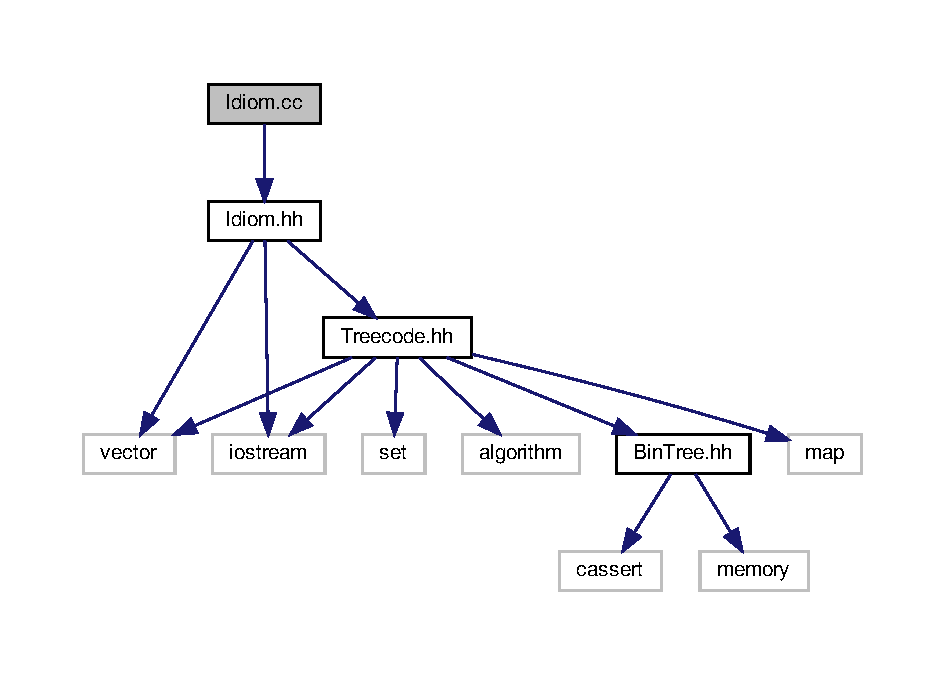
\includegraphics[width=350pt]{Idiom_8cc__incl}
\end{center}
\end{figure}


\subsection{Detailed Description}
Implementation of the \hyperlink{classIdiom}{Idiom} class. 


\hypertarget{Idiom_8hh}{}\section{Idiom.\+hh File Reference}
\label{Idiom_8hh}\index{Idiom.\+hh@{Idiom.\+hh}}


Specification for the \hyperlink{classIdiom}{Idiom} class.  


{\ttfamily \#include \char`\"{}Treecode.\+hh\char`\"{}}\newline
{\ttfamily \#include $<$vector$>$}\newline
{\ttfamily \#include $<$iostream$>$}\newline
Include dependency graph for Idiom.\+hh\+:
\nopagebreak
\begin{figure}[H]
\begin{center}
\leavevmode
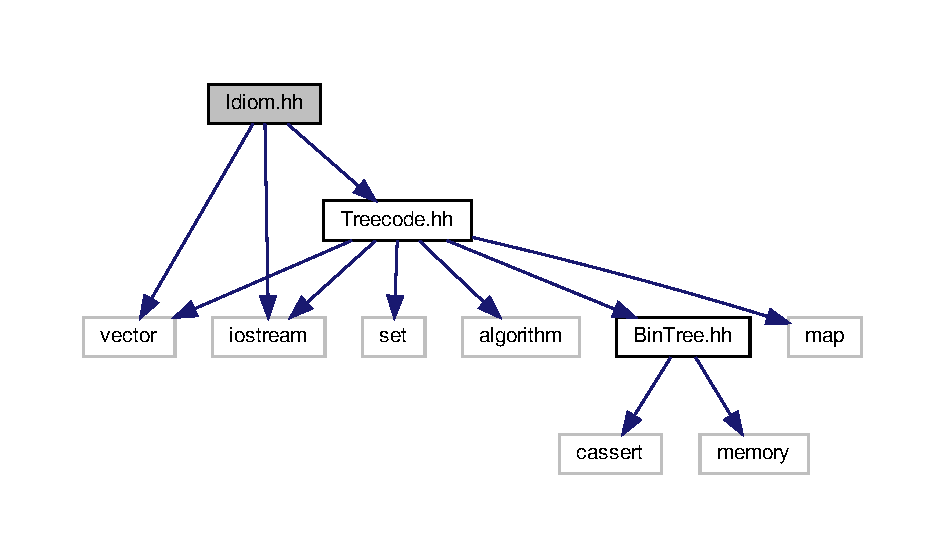
\includegraphics[width=350pt]{Idiom_8hh__incl}
\end{center}
\end{figure}
This graph shows which files directly or indirectly include this file\+:
\nopagebreak
\begin{figure}[H]
\begin{center}
\leavevmode
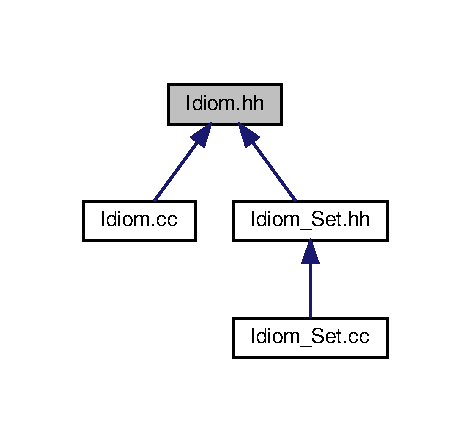
\includegraphics[width=226pt]{Idiom_8hh__dep__incl}
\end{center}
\end{figure}
\subsection*{Classes}
\begin{DoxyCompactItemize}
\item 
class \hyperlink{classIdiom}{Idiom}
\begin{DoxyCompactList}\small\item\em Represents the set of data structures and operations neded to represent our idioms. \end{DoxyCompactList}\end{DoxyCompactItemize}


\subsection{Detailed Description}
Specification for the \hyperlink{classIdiom}{Idiom} class. 


\hypertarget{Idiom__Set_8cc}{}\section{Idiom\+\_\+\+Set.\+cc File Reference}
\label{Idiom__Set_8cc}\index{Idiom\+\_\+\+Set.\+cc@{Idiom\+\_\+\+Set.\+cc}}
{\ttfamily \#include \char`\"{}Idiom\+\_\+\+Set.\+hh\char`\"{}}\newline
Include dependency graph for Idiom\+\_\+\+Set.\+cc\+:
\nopagebreak
\begin{figure}[H]
\begin{center}
\leavevmode
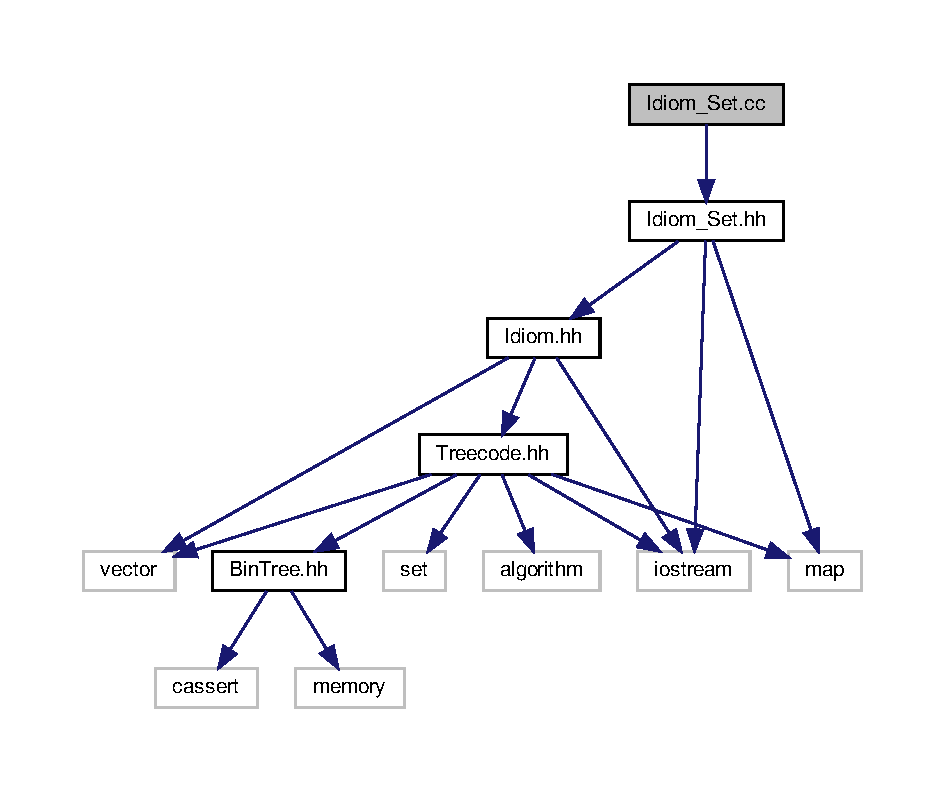
\includegraphics[width=350pt]{Idiom__Set_8cc__incl}
\end{center}
\end{figure}


\subsection{Detailed Description}
Implementation of the \hyperlink{classIdiom__Set}{Idiom\+\_\+\+Set} class 
\hypertarget{Idiom__Set_8hh}{}\section{Idiom\+\_\+\+Set.\+hh File Reference}
\label{Idiom__Set_8hh}\index{Idiom\+\_\+\+Set.\+hh@{Idiom\+\_\+\+Set.\+hh}}


Specifiction for the \hyperlink{classIdiom__Set}{Idiom\+\_\+\+Set} class.  


{\ttfamily \#include \char`\"{}Idiom.\+hh\char`\"{}}\newline
{\ttfamily \#include $<$map$>$}\newline
{\ttfamily \#include $<$iostream$>$}\newline
Include dependency graph for Idiom\+\_\+\+Set.\+hh\+:
\nopagebreak
\begin{figure}[H]
\begin{center}
\leavevmode
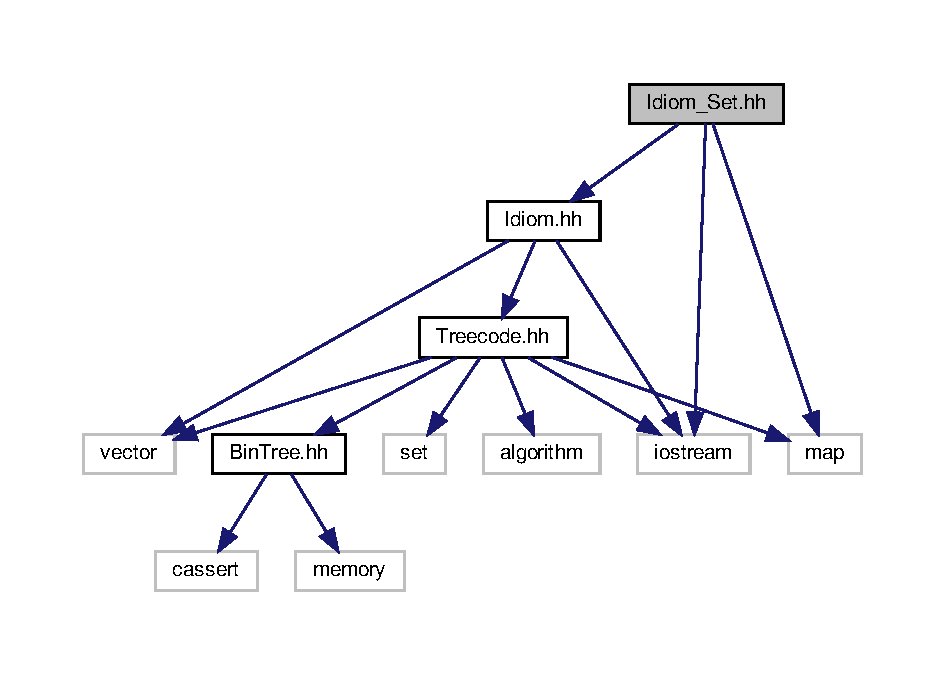
\includegraphics[width=350pt]{Idiom__Set_8hh__incl}
\end{center}
\end{figure}
This graph shows which files directly or indirectly include this file\+:
\nopagebreak
\begin{figure}[H]
\begin{center}
\leavevmode
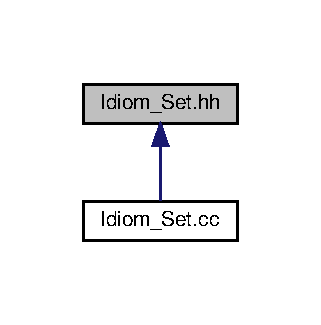
\includegraphics[width=154pt]{Idiom__Set_8hh__dep__incl}
\end{center}
\end{figure}
\subsection*{Classes}
\begin{DoxyCompactItemize}
\item 
class \hyperlink{classIdiom__Set}{Idiom\+\_\+\+Set}
\begin{DoxyCompactList}\small\item\em This class is used to store and acess multiple Idioms. \end{DoxyCompactList}\end{DoxyCompactItemize}


\subsection{Detailed Description}
Specifiction for the \hyperlink{classIdiom__Set}{Idiom\+\_\+\+Set} class. 


\hypertarget{Treecode_8cc}{}\section{Treecode.\+cc File Reference}
\label{Treecode_8cc}\index{Treecode.\+cc@{Treecode.\+cc}}


Implementation of the \hyperlink{classTreecode}{Treecode} Class.  


{\ttfamily \#include \char`\"{}Treecode.\+hh\char`\"{}}\newline
Include dependency graph for Treecode.\+cc\+:
\nopagebreak
\begin{figure}[H]
\begin{center}
\leavevmode
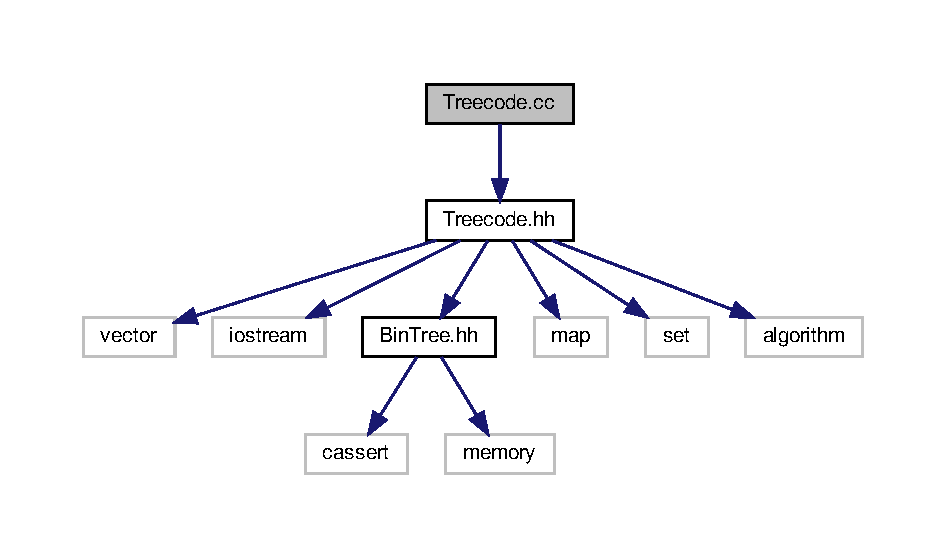
\includegraphics[width=350pt]{Treecode_8cc__incl}
\end{center}
\end{figure}
\subsection*{Functions}
\begin{DoxyCompactItemize}
\item 
\mbox{\Hypertarget{Treecode_8cc_ae11543dfb8baef265c1db56d5e7bc693}\label{Treecode_8cc_ae11543dfb8baef265c1db56d5e7bc693}} 
bool {\bfseries operator$<$} (const \hyperlink{classBinTree}{Bin\+Tree}$<$ std\+::pair$<$ std\+::string, int $>$$>$ \&t1, const \hyperlink{classBinTree}{Bin\+Tree}$<$ std\+::pair$<$ std\+::string, int $>$$>$ \&t2)
\end{DoxyCompactItemize}


\subsection{Detailed Description}
Implementation of the \hyperlink{classTreecode}{Treecode} Class. 


\hypertarget{Treecode_8hh}{}\section{Treecode.\+hh File Reference}
\label{Treecode_8hh}\index{Treecode.\+hh@{Treecode.\+hh}}


Specification for the \hyperlink{classTreecode}{Treecode} class.  


{\ttfamily \#include $<$vector$>$}\newline
{\ttfamily \#include $<$iostream$>$}\newline
{\ttfamily \#include \char`\"{}Bin\+Tree.\+hh\char`\"{}}\newline
{\ttfamily \#include $<$map$>$}\newline
{\ttfamily \#include $<$set$>$}\newline
{\ttfamily \#include $<$algorithm$>$}\newline
Include dependency graph for Treecode.\+hh\+:
\nopagebreak
\begin{figure}[H]
\begin{center}
\leavevmode
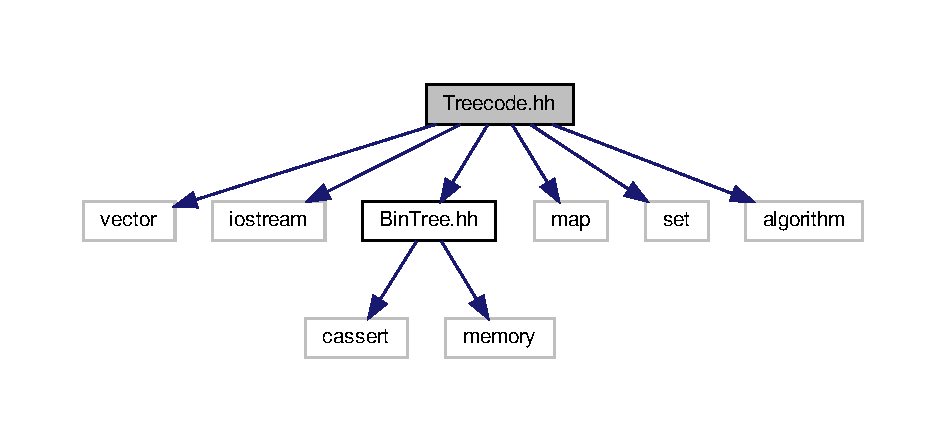
\includegraphics[width=350pt]{Treecode_8hh__incl}
\end{center}
\end{figure}
This graph shows which files directly or indirectly include this file\+:
\nopagebreak
\begin{figure}[H]
\begin{center}
\leavevmode
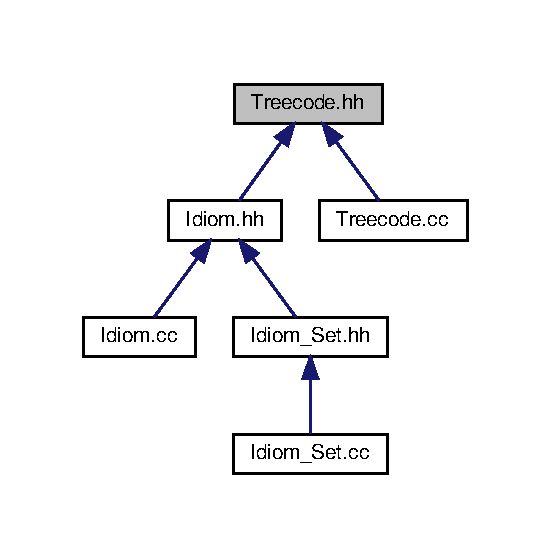
\includegraphics[width=265pt]{Treecode_8hh__dep__incl}
\end{center}
\end{figure}
\subsection*{Classes}
\begin{DoxyCompactItemize}
\item 
class \hyperlink{classTreecode}{Treecode}
\begin{DoxyCompactList}\small\item\em A class containing the data structures and operations necessary to represent our treecode. \end{DoxyCompactList}\end{DoxyCompactItemize}


\subsection{Detailed Description}
Specification for the \hyperlink{classTreecode}{Treecode} class. 


%--- End generated contents ---

% Index
\backmatter
\newpage
\phantomsection
\clearemptydoublepage
\addcontentsline{toc}{chapter}{Index}
\printindex

\end{document}
